%!TEX TS-program = xelatex
\documentclass{friggeri-cv}
\usepackage{afterpage}
\usepackage{hyperref}
\usepackage{color}
\usepackage{xcolor}
\hypersetup{
	pdftitle={},
    pdfauthor={},
    pdfsubject={},
    pdfkeywords={},
    colorlinks=false,       % no lik border color
   allbordercolors=white    % white border color for all
}
\addbibresource{bibliography.bib}
\RequirePackage{xcolor}
\definecolor{pblue}{HTML}{0395DE}
\begin{document}
\header{Guillaume Le Roux} {}
	{Computer Engineer}

	% Fake text to add separator      
\fcolorbox{white}{gray}{\parbox{\dimexpr\textwidth-2\fboxsep-2\fboxrule}{%
	.....
}}

\begin{aside}
	
\includegraphics[scale=1] {profil.png}
\section{Address}
	16, Kergaigne
	44350 Guerande
	France
	~
	\section{Tel}
	+336 75 94 39 92
	~
	\section{Mail}
	\href{mailto:guillaume@leroux.email}{\textbf{guillaume@}\\leroux.email}
	~
	\section{Programming}
	
\includegraphics[scale=0.40]{img/5stars.png}\\\textbf{Php, Symfony, HTML, CSS, SQL, git}
	
\includegraphics[scale=0.40]{img/4stars.png}\\\textbf{Java, Javascript, Apache2}
	
\includegraphics[scale=0.40]{img/3stars.png}\\\textbf{ReactJs, Go}
	
\includegraphics[scale=0.40]{img/2stars.png}\\\textbf{VueJs, C++}
	~
	\section{OS Preference}
	\textbf{Linux}
\includegraphics[scale=0.40]{img/5stars.png}
	\textbf{Windows}
\includegraphics[scale=0.40]{img/2stars.png}
	~
	\section{Personal skills}
	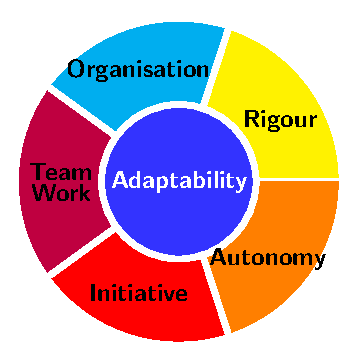
\includegraphics[scale=0.70]{test.pdf}
	~
	\section{Languages}
	\textbf{French}
\includegraphics[scale=0.40]{img/5stars.png}
	\textbf{English}
\includegraphics[scale=0.40]{img/4stars.png}
	\textbf{Breton}
\includegraphics[scale=0.40]{img/4stars.png}
\end{aside}

\section{Description}
\begin{entrylist}
	I am looking for a job as back end developper \\
	After two years of experience as Full Stack-Web developper, in Smile Open Source Solutions \\
	In order to improve my English I am looking for a job in an english speaker country \\	
\end{entrylist}

\section{Experience}
\begin{entrylist}
	\entry
	{03/17 - Now}
	{Software Engineer}
	{Smile Open Source Solutions}
	{
		For Smile I have mainly worked for four differents customer : \\
		\\
		\textbf{Trigano} : First french constructor of camper and caravan \\
			In a team of three we made the front of their intranet using ReactJs and consuming API's \\
		\textbf{Elephorm} : Theyproduce and sells online lessons on various topics \\ 
			Initiated the rework of their website for four month in Symfony. \\
			In a team of four developper in an agil process, we set up a stack of continuous development with a Jenkins, we used code review and differents qualtity tools to have quality reference. \\
		\textbf{Suez} : A world leader in sustainable resource management \\
				I made a POC for a Progressive Web App with a front in ReactJs and a Back in Go \\
				For this POC i was in autonomy with a direct relation with the customer \\
		\textbf{Axelliance} : Second french broker wholesealer in insurance \\
			In a team of four developper we were in charge of developping and launching new website and existing park maintenance \\
			we had to work with a product owner who create the specifications in an agile process 
	}
\end{entrylist}

\section{Education}
\begin{entrylist}
	\entry
	{2014 - 2017}
	{Master's Degree in Computer Engineering}
	{Université Rennes 1 - France}
	{Main subjects : Algorithms, Object Oriented Programming, Design paterns. \\
	During this graduation we had to do several projects using differents languages \\
	such as a text Editor in Java, client/server music streaming in C, an asteroid game in OCaml, ...
	}
	\entry
	{2011 - 2014}
	{Bachelor's degree \\in Applied Mathematics ans Social Sciences }
	{Université Rennes 2 - France}
	{Main subjects: Mathematics such as aglebra, probabilitys, statistics and enconomy.}
\end{entrylist}
\section{Hobbies}
\begin{entrylist}
	\entry  {} {Sailing as skipper} {}
	{
		For many years i went to sailing, with a crew of four to six sailors. \\
		During one to two weeks cruise i had to manage different situations
	}
	\entry  {} {Sports, Handball in club} {} {I have been playing Handball for ten years, in differents club}
\end{entrylist}

\end{document}
